\documentclass{article}

\usepackage[%
    left=0.5in,%
    right=0.5in,%
    top=0.5in,%
    bottom=0.5in,%
]{geometry}%
\usepackage{minitoc}
\usepackage{multicol}
\usepackage{graphicx}
\usepackage{fixltx2e}
\usepackage{listings}
\usepackage{color}
\usepackage{hyperref}
    \hypersetup{ colorlinks = true, linkcolor = blue }
\usepackage{blindtext}
\definecolor{lightgray}{gray}{0.9}
\graphicspath{ {./} }

\newcommand{\inlinecode}[2]{\colorbox{lightgray}{\lstinline
[language=#1]$#2$}}
\newcommand{\worddef}[1]{\hyperref[sec:reference]{\textit{#1}}}

\begin{document}

\tableofcontents

\newpage

\section{Definition}

\begin{flushleft}
Software testing is a formal process carried out by a \textbf{specialized testing team} in which a software unit, several integrated software units or an entire software package are examined by running the programs on a computer.
\end{flushleft}

\section{Objectives}

\begin{flushleft}
Direct objectives
\begin{itemize}
  \item To identify and reveal as many errors as possible in the tested software
  \item To bring the tested software, after correction of the identified errors and retesting, to an acceptable level of quality
  \item To perform the required tests efficiently and effctively, within the limits budgetary and scheduling limitations
\end{itemize}
Indirect objectives
\begin{itemize}
  \item To compile a record of software errors for use in error prevention (by corrective and preventive actions)
\end{itemize}
\end{flushleft}

\section{Strategic approach to testing}

\subsection{General characteristics}
\begin{itemize}
  \item Software team should conduct effective formal technical reviews
  \item Testing begins at the component level and work outward toward the integration of the whole system
  \item Testing is conducted by the \textbf{developer} of the software and by \textbf{independent test group}.
  \item Testing and debugging are different activities, but debugging must be accomodated in any testing strategy.
\end{itemize}

\subsection{Verification and validation}

\begin{itemize}
  \item Verification: (Are algorithms coded correctly?). The set of activities that ensure that software corrctly implements specfic function or algorithm.
  \item Validation (Does it meet user requirements). The set of activities that ensure that the software that has been build is traceable to customer requirements.
\end{itemize}

\subsection{Organising software testing}
Testing should aim at breaking the software
\begin{itemize}
  \item Independent test group
  \begin{itemize}
    \item Removes the inherent problems asociation with letting the builder test the software that has been built
    \item Removes the conflict of interest that may otherwise be present
    \item Works closely with the software developer during analysis and design to ensure that throughout testing occues.
  \end{itemize}
\end{itemize}

\subsection{Levels of testing}

\begin{itemize}
  \item Unit testing: Concentratest on each component/function of the software as implemented in source code
  \begin{itemize}
    \item Exercises specific paths in a component's control structure to ensure complete coverage and maximum error detection.
    \item Components are then assembled and integrated
  \end{itemize}
  \item Integration testing: Focuses on the design and construction of the software architecture
  \begin{itemize}
    \item Focuses on inputs and outputs, and how well components fit and work together
  \end{itemize}
  \item Validation testing: Requirements are validated against each constructed software
  \begin{itemize}
    \item Provides final assurance that the software meets all functional, behaviour, and performance requirements
  \end{itemize}
  \item System testing: The software and other system elements are tested as a whole
  \begin{itemize}
    \item Verifies that all system elements (software, hardware, people, databases) mesh properly and that overall system function and performance is achieved
  \end{itemize}
\end{itemize}

\begin{center}
  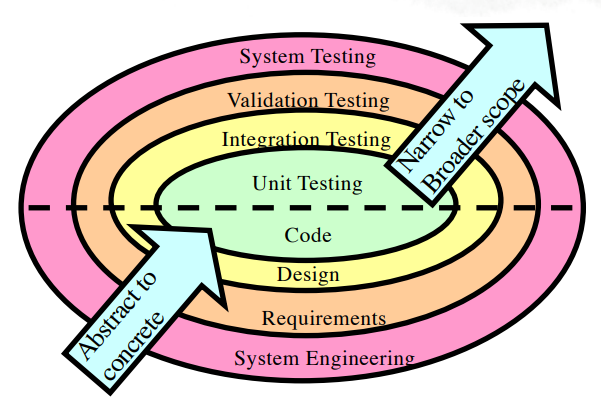
\includegraphics[scale=0.5]{testing_strategy.png}
\end{center}

\subsection{Testing strategy appliet to Object-Oriented Software}

\begin{itemize}
  \item Include detections of errors in analysis and design models
  \item Unit testing loses some of its meaning and integration testing changes signifcantly
  \item Use the same philosophy but different approach as in conventional software testing
  \item Test "in the smal" and the work out to testing "in the large"
  \begin{itemize}
    \item Testing in the small involves class attrivutes and operations, main focus in on communication and collaboration within the class
    \item Testing in the large involves a series of regression tests to uncover errors due to communication and collabolration among classes
  \end{itemize}
  \item Finally, the system as a whole is tested to detect errors in fulfilling requirements
\end{itemize}

\section{Ensuring a successful software test strategy}

\begin{itemize}
  \item Specify product requirements in a \textbf{quantifiable} manner long before testing commences
  \item State testing objectives explicitly in measurable terms
  \item Understand the user of the software (through use cases) and develop a profile for each user category
  \item Develop a testing plan that emphasizes rapid cycle testing to get quick feedback to control quality levels and adjust the test strategy
  \item Build robust software that is designed to test itself and can diagnose certain kinds of errors
  \item Use effective formal technical reviews as a filter prior to testing to reduce the amount of testing required
  \item Conduct formal technical reviews to asses the test strategy and test casess themselves
  \item Develop a continous improvement approach for the testing process through the gathering of metrics
\end{itemize}

\pagebreak

\section{Defect testing}

\begin{quote}
A successful defect test is a test which causes a program to behave in an anomalous way. Tests show the presence not the absence of defects
\end{quote}

\subsection{The testing process}
\begin{flushleft}
Component testing
\begin{itemize}
  \item Testing of individual program components
  \item Usually the responsiblity of the component developer (except for critical systems)
  \item Tests are derived for the developers experience
\end{itemize}
Integration testing
\begin{itemize}
  \item Testing of groups of components integrated to create a system or a sub-system
  \item The responsibility of an independent testing team
  \item Tests are based on a system specification
\end{itemize}
\end{flushleft}

\subsection{Testing priorities}

\begin{itemize}
  \item Only exhaustive testing can show a program is free from defects
  \item Test should exercise a system's capabilities rather than its components
  \item Testing old capabilities is more important than testing new capabilities. In order for compatability purposes.
  \item Testing typical situations is more important than boundary value cases.
\end{itemize}

\begin{center}
  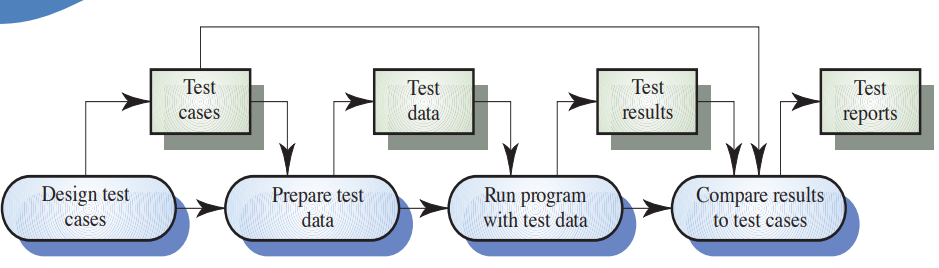
\includegraphics[scale=0.5]{defect_testing.png}
\end{center}

\section{Black box testing}

\begin{itemize}
  \item An approach to testing where the program is considered as a black-box
  \item The program test cases are based on the system specification 
  \item Test planning can begin \textbf{early} in the software process as we don't need to test the internals, just the visible output
\end{itemize}

\section{Equivalence partitioning}

\begin{itemize}
  \item Input data and output results often fall into different classes where all members of a class are related 
  \item Each of these classes is an \worddef{equivalence partition} where the program behaves in an equivalent way for each class member 
  \item Test cases should be chosen from each partition
\end{itemize}

\subsection{Binary search equivalence partitions}

\begin{itemize}
  \item Pre-conditions satisfied, key element in array 
  \item Pre-conditions satisfied, key element not in array 
  \item Pre-conditions unsatisfied, key element in array 
  \item Pre-conditions unsatisfied, key element not in array 
  \item Input array has a single value 
  \item Input array has an even number of values 
   Input array has an odd number of values
\end{itemize}

\subsection{Testing guidelines (sequences)}

\begin{itemize}
  \item Test software with sequences which have only a single value
  \item Use sequences of different sizes in different tests
  \item Derive tests so that the first, middle and last elements of the sequence are accessed
  \item Test with sequences of zero length
\end{itemize}

\subsection{Equivalence class Test cases}

\begin{flushleft}
According to the equivalence class (EC) partitioning method:
\end{flushleft}
\begin{itemize} 
  \item Each \textbf{valid} EC and each \textbf{invalid} EC are included in at least one test case. With definitions made separately.
  \item In defining a test case for the valid ECs, we try to cover as many as possible “new” ECs in that same test case. 
  \item In defining invalid ECs, we must assign one test case to \textbf{each “new” invalid EC}, as a test case that includes more than one invalid EC may not allow the tester to distinguish between the program’s separate reactions to each of the invalid ECs. 
  \item Test cases are added as long as there are uncovered ECs.
\end{itemize}

\section{Structural testing}

\begin{itemize}
  \item Sometimes called \textbf{white-box} testing 
  \item Derivation of test cases according to program structure. Knowledge of the program is used to identify additional test cases 
  \item Objective is to exercise all program statements (not all path combinations)
\end{itemize}

\begin{center}
  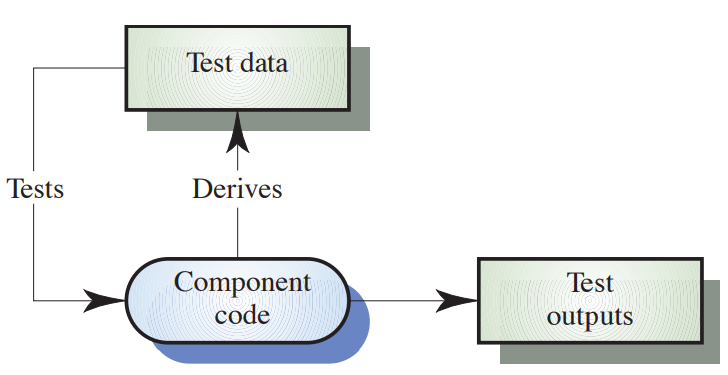
\includegraphics[scale=0.5]{white_box_testing.png}
\end{center}

\section{Path testing}
\begin{itemize}
  \item Ensure that the set of test cases is such that each path through the program is executed at least once 
  \item The starting point for path testing is a program flow graph that shows nodes representing program decisions and arcs representing the flow of control 
  \item Statements with conditions are therefore \textbf{nodes} in the flow graph
\end{itemize}

\subsection{Program flow graphs}

\begin{itemize}
  \item Describes the program control flow. Each branch is shown as a separate path and loops are shown by arrows looping back to the loop condition node 
  \item This is also used as a basis for computing the cyclomatic complexity 
  \item Cyclomatic complexity = Number of edges - Number of nodes +2
\end{itemize}

\subsection{Cyclomatic complexity}

\begin{itemize}
  \item The number of tests to \textbf{test all control statements} equals the \textit{cyclomatic complexity} 
  \item Cyclomatic complexity equals number of conditions in a program 
  \item Useful if used with care. Does not imply adequacy of testing. 
  \item Although all paths are executed, \textbf{all combinations} of paths are not executed
\end{itemize}

\begin{center}
  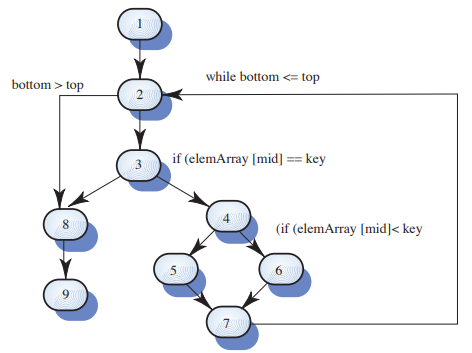
\includegraphics[scale=0.5]{search_flow_graph.png}
\end{center}

\section{Path vs Line coverage}

\begin{flushleft}
\textbf{Path coverage} of a test is measured by the percentage of all possible program paths included in planned testing. \textbf{Line coverage} of a test is measured by the percentage of program code lines included in planned testing.
\end{flushleft}

\section{Integration testing}

\begin{itemize}
  \item Tests \textbf{complete systems} or subsystems composed of integrated components 
  \item Integration testing should be black-box testing with tests derived from the specification 
  \item Main difficulty is localising errors 
  \item \textbf{Incremental integration} testing reduces this problem
\end{itemize}

\begin{center}
  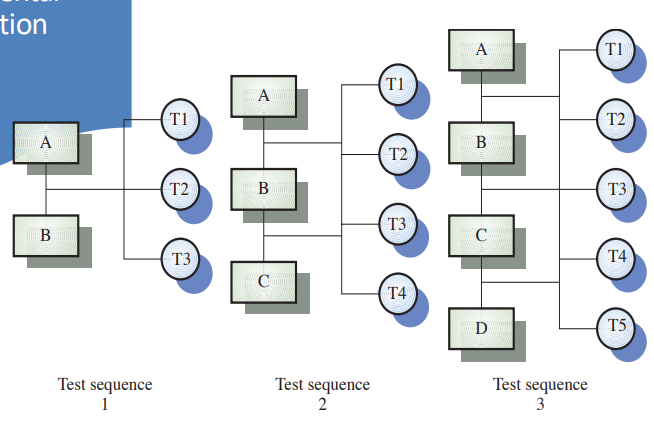
\includegraphics[scale=0.5]{inc_integration_testing.png}
\end{center}

\subsection{Approaches to integration testing}

\begin{itemize}
  \item \textbf{Top-down testing} – Start with high-level system and integrate from the top-down replacing individual components by stubs where appropriate 
  \item \textbf{Bottom-up testing} – Integrate individual components in levels until the complete system is created 
  \item In practice, most integration involves a combination of these strategies
\end{itemize}

\subsection{Testing approaches}

\begin{itemize}
  \item \textbf{Architectural validation} – Top-down integration testing is better at discovering errors in the system architecture 
  \item \textbf{System demonstration} – Top-down integration testing allows a limited demonstration at an early stage in the development 
  \item \textbf{Test implementation} – Often easier with bottom-up integration testing 
  \item \textbf{Test observation} – Problems with both approaches. Extra code may be required to observe tests
\end{itemize}

\section{Interface testing}

\begin{itemize}
  \item Takes place when modules or sub-systems are integrated to create larger systems 
  \item Objectives are to detect faults due to interface errors or invalid assumptions about interfaces 
  \item Particularly important for \textbf{object-oriented} development as objects are defined by their interfaces
\end{itemize}

\subsection{Interface types}
    
\begin{itemize}
  \item \textbf{Parameter interfaces} – Data passed from one procedure to another 
  \item \textbf{Shared memory interfaces} – Block of memory is shared between procedures 
  \item \textbf{Procedural interfaces} – Sub-system encapsulates a set of procedures to be called by other sub-systems 
  \item \textbf{Message passing interfaces} – Sub-systems request services from other sub-systems
\end{itemize}

\subsection{Interface errors}

\begin{itemize}
  \item \textbf{Interface misuse} – A calling component calls another component and makes an error in its use of its interface e.g. parameters in the wrong order 
  \item \textbf{Interface misunderstanding} – A calling component embeds assumptions about the behaviour of the called component which are incorrect 
  \item \textbf{Timing errors} – The called and the calling component operate at different speeds and out-of-date information is accessed
\end{itemize}

\subsection{Interface testing guidelines}

\begin{itemize}
  \item Design tests so that parameters to a called procedure are at the \textbf{extreme ends of their ranges} 
  \item Always test pointer parameters with null pointers 
  \item Design tests which cause the component to fail 
  \item Use stress testing in message passing systems 
  \item In shared memory systems, vary the order in which components are activated
\end{itemize}

\section{Stress testing}

\begin{itemize}
  \item Exercises the system beyond its maximum design load. Stressing the system often causes defects to come to light 
  \item Stressing the system test failure behaviour.. Systems should not fail catastrophically. Stress testing checks for unacceptable loss of service or data 
  \item Particularly relevant to distributed systems which can exhibit severe degradation as a network becomes overloaded
\end{itemize}

\section{Object-oriented testing}

\begin{itemize}
  \item The components to be tested are object classes that are instantiated as objects 
  \item Larger grain than individual functions so approaches to white-box testing have to be extended 
  \item No obvious ‘top’ to the system for top-down integration and testing
\end{itemize}

\subsection{Testing levels}

\begin{itemize}
  \item Testing operations associated with objects 
  \item Testing object classes 
  \item Testing clusters of cooperating objects 
  \item Testing the complete OO system
\end{itemize}

\subsection{Object class testing}

\begin{itemize}
  \item Complete test coverage of a class involves – Testing all operations associated with an object – Setting and interrogating all object attributes – Exercising the object in all possible states 
  \item Inheritance makes it more difficult to design object class tests as the information to be tested is not localised
\end{itemize}

\subsection{Object integration}

\begin{itemize}
  \item Levels of integration are less distinct in object-oriented systems
  \item Cluster testing is concerned with integrating and testing clusters of cooperating objects
  \item Identify clusters using knowledge of the operation of objects and the system features that
are implemented by these cluster
\end{itemize}

\section{Approaches to cluster testing}

\begin{itemize}
  \item Use-case or scenario testing
  \begin{itemize}
    \item Testing is based on a user interactions with the system
    \item Has the advantage that it tests system features as experienced by users 
  \end{itemize}
  \item Thread testing – Tests the systems response to events as processing threads through the system 
  \item Object interaction testing: Tests sequences of object interactions that stop when an object operation does not call on services from another object
\end{itemize}

\section{Scenario based testing}

\begin{itemize}
  \item Identify scenarios from use-cases and supplement these with interaction diagrams that show the objects involved in the scenario
  \item Consider the scenario in the weather station system where a report is generated
\end{itemize}

\section{Debugging}

\begin{itemize}
  \item The debugging process begins with the execution of a test case 
  \item Results are assessed and the difference between expected and actual performance is encountered 
  \item This difference is a symptom of an underlying cause that lies hidden
  \item The debugging process attempts to match symptom with cause, thereby leading to error correction
\end{itemize}

\subsection{Why is it difficult}

\begin{itemize}
  \item The symptom and the cause may be geographically remote
  \item The symptom may disappear (temporarily) when another error is corrected 
  \item The symptom may actually be caused by nonerrors(e.g., round-off accuracies) 
  \item The symptom may be caused by human error that is not easily traced
  \item The symptom and the cause may be geographically remote 
  \item The symptom may disappear (temporarily) when another error is corrected 
  \item The symptom may actually be caused by nonerrors(e.g., round-off accuracies) 
  \item The symptom may be caused by human error that is not easily traced
\end{itemize}

\subsection{Debugging strategies}

\begin{itemize}
  \item Objective of debugging is to \textbf{find and correct the cause of a software error}
  \item Debugging methods and tools are not a substitute for careful evaluation based on a
complete design model and clear source code.
\end{itemize}

\subsubsection{Brute forcing}

\begin{itemize}
  \item Most commonly used and least efficient method 
  \item Used when all else fails 
  \item Involves the use of memory dumps, run-time traces, and output statements 
  \item Leads many times to wasted effort and time
\end{itemize}

\subsubsection{Backtracing}

\begin{itemize}
  \item Can be used successfully in small programs 
  \item The method starts at the location where a symptom has been uncovered 
  \item The source code is then traced backward (manually) until the location of the cause is found 
  \item In large programs, the number of potential backward paths may become unmanageably large
\end{itemize}

\subsubsection{Cause elimination}

\begin{itemize}
  \item Involves the use of induction or deduction and introduces the concept of binary partitioning
  \begin{itemize}
    \item Induction (specific to general): Prove that a specific starting value is true; then prove the general case is true
    \item Deduction (general to specific): Show that a specific conclusion follows from a set of general premises 
  \end{itemize}
  \item Data related to the error occurrence are organized to isolate potential causes 
  \item A cause hypothesis is devised, and the aforementioned data are used to prove or disprove the hypothesis 
  \item Alternatively, a list of all possible causes is developed, and tests are conducted to eliminate each cause 
  \item If initial tests indicate that a particular cause hypothesis shows promise, data are refined in an attempt to isolate the bug
\end{itemize}

\section{Key points}

\begin{itemize}
  \item Test parts of a system which are commonly used rather than those which are rarely executed 
  \item Equivalence partitions are sets of test cases where the program should behave in an equivalent way 
  \item Black-box testing is based on the system specification 
  \item Structural testing identifies test cases which cause all paths through the program to be executed
  \item Test coverage measures ensure that all statements have been executed at least once. 
  \item Interface defects arise because of specification misreading, misunderstanding, errors or invalid timing assumptions 
  \item To test object classes, test all operations, attributes and states 
  \item Integrate object-oriented systems around clusters of objects
\end{itemize}

\pagebreak
\section*{Reference section} \label{sec:reference}
\begin{description}
	\item[equivalence partitioning] \hfill \\ Equivalence partitioning or equivalence class partitioning (ECP) is a software testing technique that divides the input data of a software unit into \textbf{partitions of equivalent data from which test cases can be derived}. In principle, test cases are designed to cover each partition at least once.
\end{description}
\end{document}
